\chapter{Results}

\subsection{Dataset}
In order to complete this letter frequncy analysis through Hadoop, several datasets of different sizes were used. 

The smallest datasets are about the theatrical piece \textit{Seagull} by Anton Chekhov. Each file is approximately 100KB and includes: 
\begin{itemize}
    \item The English translation
    \item The Italian translation
    \item The Turkish translation
\end{itemize}

The medium datasets are about the \textit{Lord Of The Rings} trilogy by J.R.R. Tolkien. Each file is approximately 3MB and includes: 
\begin{itemize}
    \item The original English text
    \item The Italian translation
    \item The Turkish translation
\end{itemize}

The largest dataset is a collection of 5 Million book reviews in English from Goodreads. This dataset is about 3GB. 
 
The datasets are stored in HDFS and were processed by the Hadoop MapReduce framework. The results of the analysis were stored in HDFS and were later retrieved and analyzed.
\newpage
\section{Performance}
The performance of the Hadoop MapReduce framework was tested on the English datasets. This allowed us to see the difference peformances for the different sizes with the different number of reducers and the use of the different algorithms.
\begin{figure}[h]
    \centering
    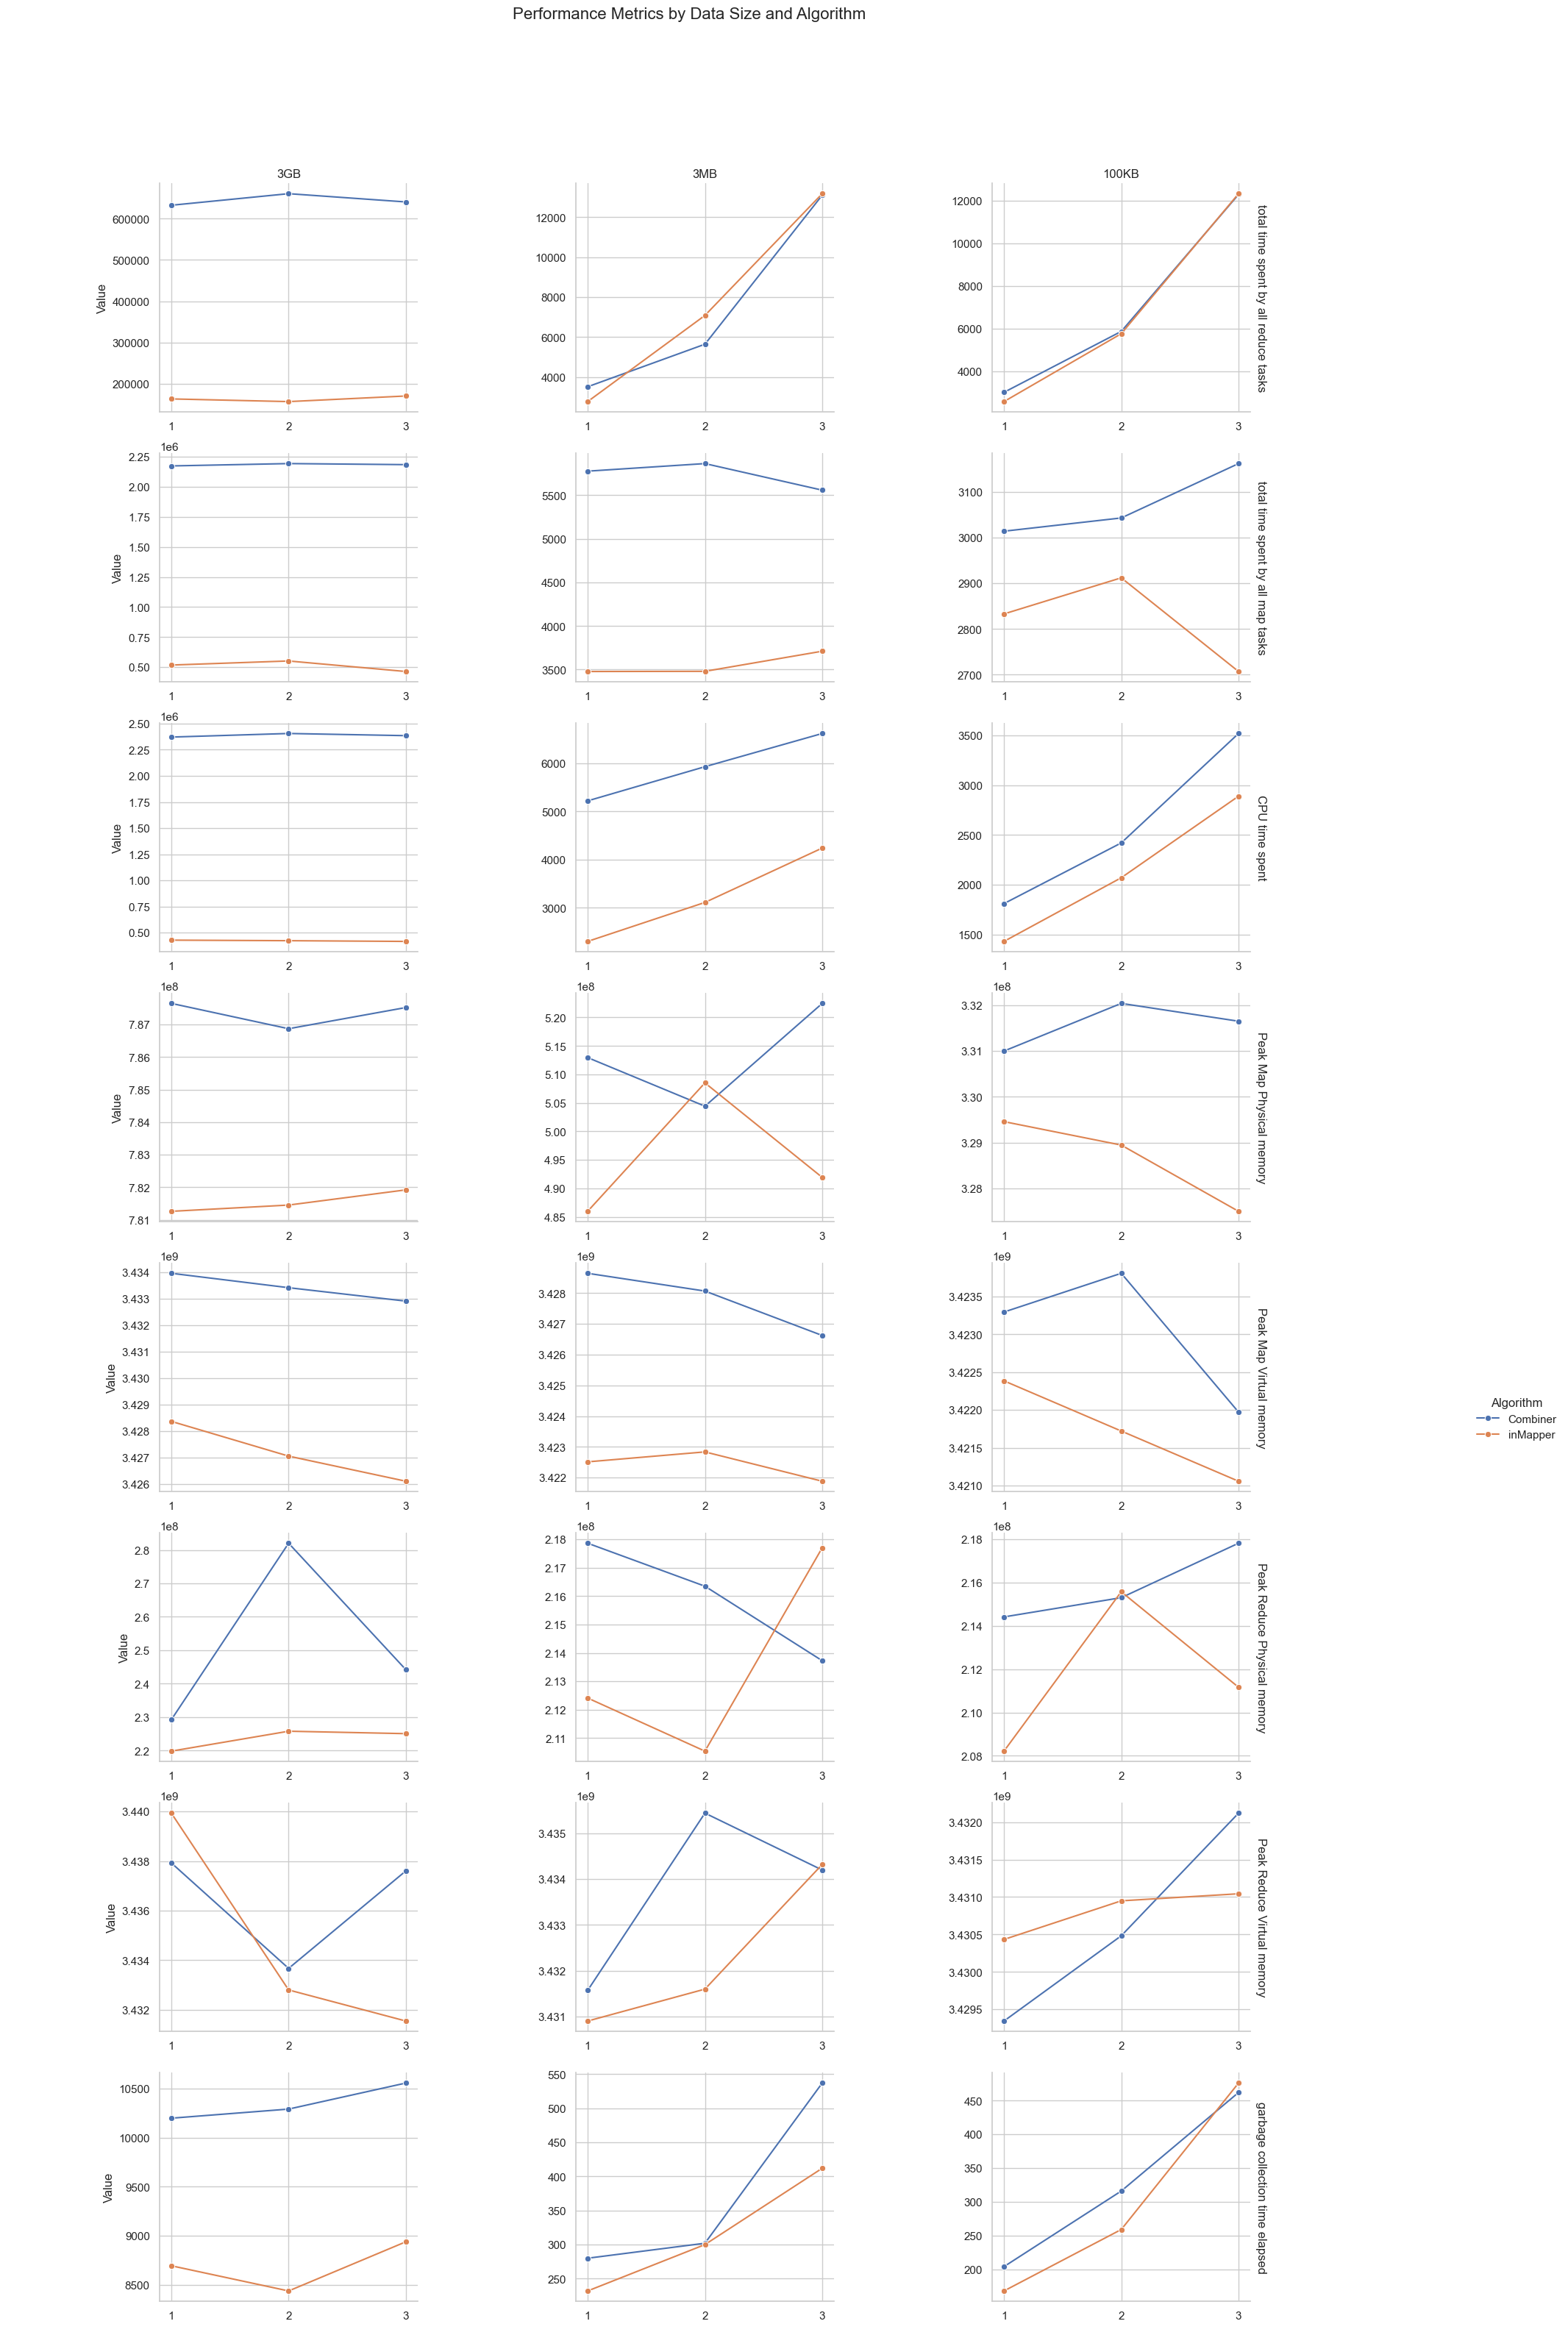
\includegraphics[width=1\textwidth]{media/performance_graph_cut.png}
\end{figure}

\textbf{Obtained Results:}
\subsection{Total Time Spent by All Reduce Tasks}
\begin{itemize}
    \item \textbf{100KB}: Both algorithms show similar performance with slight differences as the number of reducers increases. The Combiner algorithm tends to have a slightly higher total time.
    \item \textbf{3MB}: Both algorithms again show similar trends, but \textit{inMapper} has a slight edge in performance, especially as the number of reducers increases.
    \item \textbf{3GB}: \textit{inMapper} shows a slight increase in total time with more reducers, while Combiner shows more fluctuation but remains generally higher.
\end{itemize}

\subsection{Total Time Spent by All Map Tasks}
\begin{itemize}
    \item \textbf{100KB}: Both algorithms have similar trends, with slight fluctuations.
    \item \textbf{3MB}: \textit{inMapper} tends to perform slightly better with an increasing number of reducers.
    \item \textbf{3GB}: Similar to the reduce tasks, \textit{inMapper} generally performs better, though the performance gap narrows with more reducers.
\end{itemize}

\subsection{CPU Time Spent}
\begin{itemize}
    \item \textbf{100KB and 3MB}: \textit{inMapper} consistently shows lower CPU time spent compared to Combiner, indicating better efficiency.
    \item \textbf{3GB}: The trend is similar, with \textit{inMapper} being more efficient as the number of reducers increases.
\end{itemize}

\subsection{Peak Map Physical Memory}
\begin{itemize}
    \item \textbf{100KB}: Memory usage is relatively stable across reducers, with slight variations.
    \item \textbf{3MB}: Both algorithms show an increase in memory usage with more reducers, but \textit{inMapper} has slightly lower memory usage.
    \item \textbf{3GB}: Similar trends with \textit{inMapper} showing better memory efficiency.
\end{itemize}

\subsection{Peak Map Virtual Memory}
\begin{itemize}
    \item The trends are similar across all sizes, with \textit{inMapper} generally having slightly better performance (lower values) than Combiner.
\end{itemize}

\subsection{Peak Reduce Physical Memory}
\begin{itemize}
    \item \textbf{100KB}: Both algorithms have similar trends, with slight fluctuations.
    \item \textbf{3MB}: \textit{inMapper} shows better memory efficiency as the number of reducers increases.
    \item \textbf{3GB}: Similar trends with \textit{inMapper} being more efficient.
\end{itemize}

\subsection{Peak Reduce Virtual Memory}
\begin{itemize}
    \item Similar to physical memory, \textit{inMapper} generally shows better performance across all sizes.
\end{itemize}

\subsection{Garbage Collection Time Elapsed}
\begin{itemize}
    \item \textbf{100KB}: Both algorithms have similar trends, with slight differences.
    \item \textbf{3MB and 3GB}: \textit{inMapper} generally shows lower garbage collection times, indicating better memory management.
\end{itemize}


In analyzing the performance of the two algorithms (Combiner and inMapper) across different data sizes (100KB, 3MB, 3GB) and varying numbers of reducers (1, 2, 3), several trends emerge:

\begin{itemize}
    \item \textbf{Efficiency and Resource Usage}: The \textit{inMapper} algorithm consistently demonstrates better efficiency across multiple metrics, including CPU time, physical and virtual memory usage, and garbage collection times. This indicates that \textit{inMapper} handles tasks more effectively, especially with larger data sizes.
    \item \textbf{Scalability with Reducers}: Both algorithms benefit from an increased number of reducers, though \textit{inMapper} shows more significant performance gains. This suggests that \textit{inMapper} scales better with additional resources.
    \item \textbf{Performance with Larger Data Sizes}: As data size increases, the performance difference between the algorithms becomes more apparent. \textit{inMapper} generally outperforms Combiner, particularly with larger datasets (3GB), making it a preferable choice for large-scale data processing tasks.
\end{itemize}

Overall, the \textit{inMapper} algorithm proves to be more efficient and scalable, particularly when dealing with larger datasets and an increasing number of reducers. This makes it a better choice for high-performance data processing scenarios.


\newpage

\section{Frequency}
The frequency of the letters was tested in English, Italian and Turkish using the small (Seagull) and medium (Lord of the Rings) datasets. 
This allowed to compare frequency differences between the languages and the different sizes datasets.\\ \\
Below it can be seen the results of the frequency analysis for the small and medium datasets for each languages.

\begin{figure}[h]
    \centering
    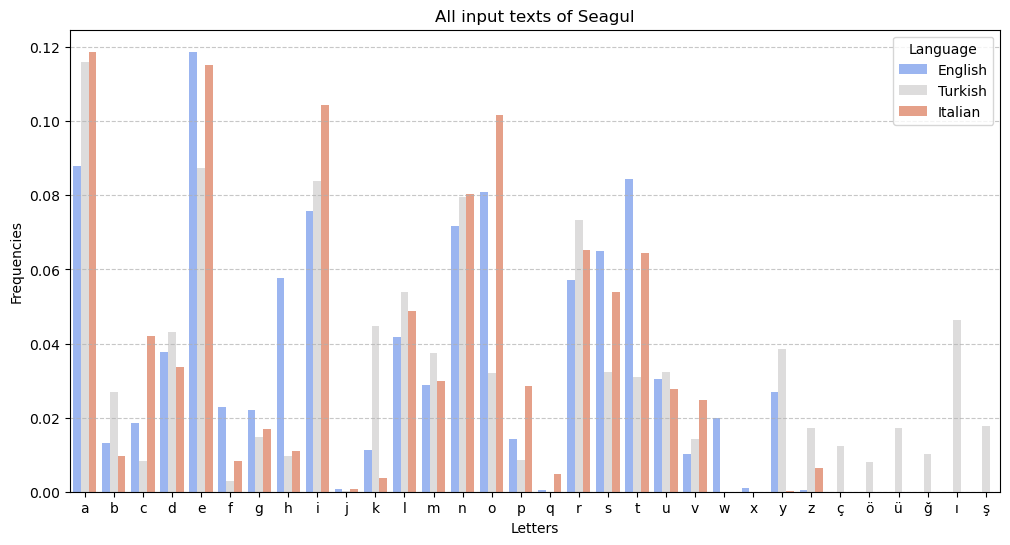
\includegraphics[width=1\textwidth]{media/allSeagul.png}
\end{figure}

\begin{figure}[h]
    \centering
    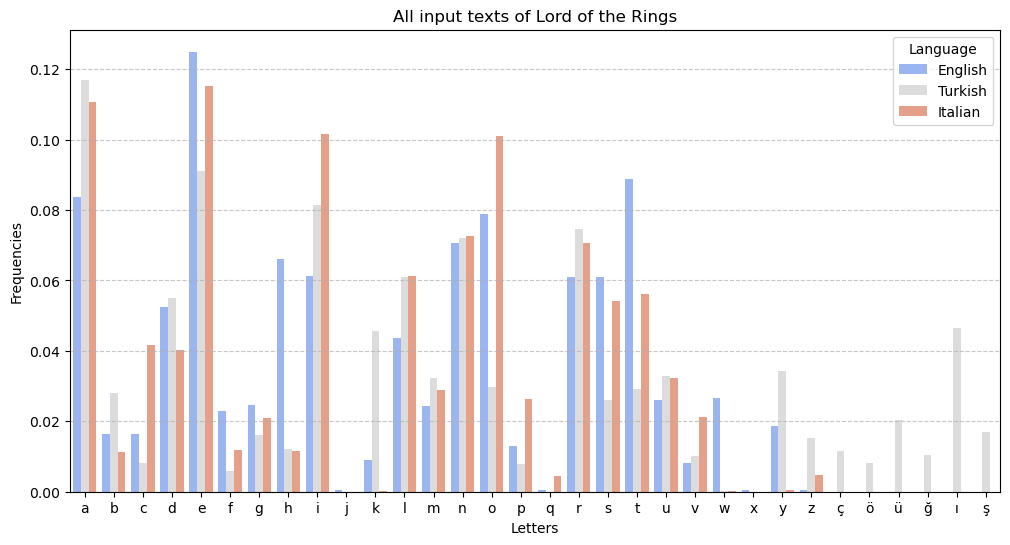
\includegraphics[width=1\textwidth]{media/allLordOfTheRings.png}
\end{figure}

\newpage

\subsection*{Letter frequency results for all datasets in each languages separately} 

\begin{figure}[htbp]
    \centering
    \begin{minipage}[b]{0.45\textwidth}
        \centering
        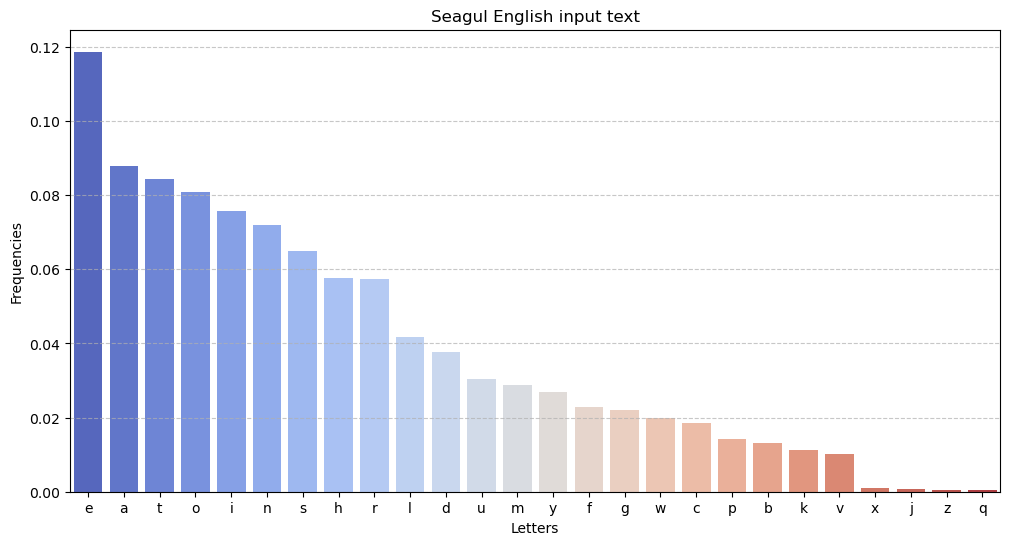
\includegraphics[width=\textwidth]{media/seagulEnglish.png} 
        \caption{Letter Frequency of Seagul in English}
    \end{minipage}
    \hfill
    \begin{minipage}[b]{0.45\textwidth}
        \centering
        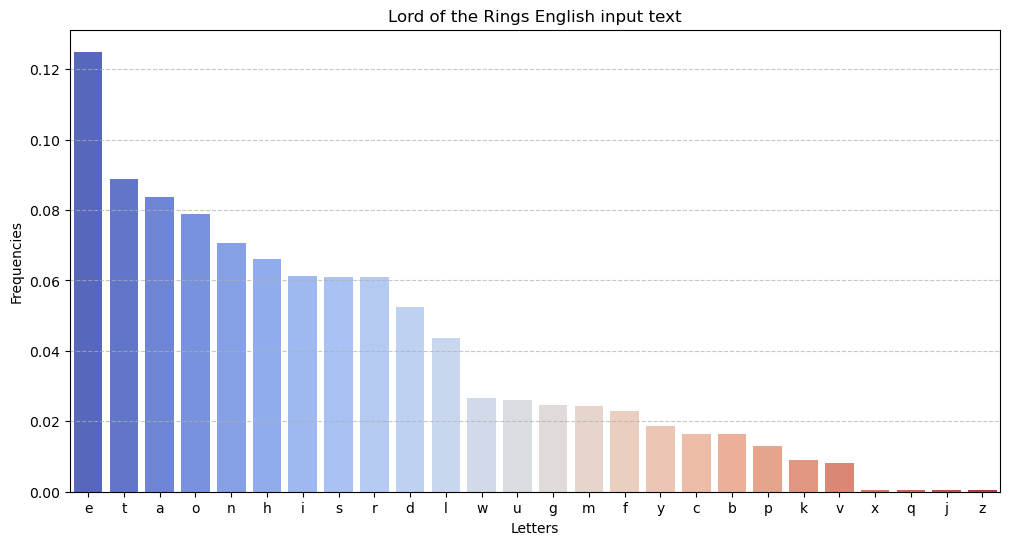
\includegraphics[width=\textwidth]{media/lordOfTheRingsEnglish.png}
        \caption{Letter Frequency of Lord of the Rings in English}
    \end{minipage}
\end{figure}

\begin{figure}[htbp]
    \centering
    \begin{minipage}[b]{0.45\textwidth}
        \centering
        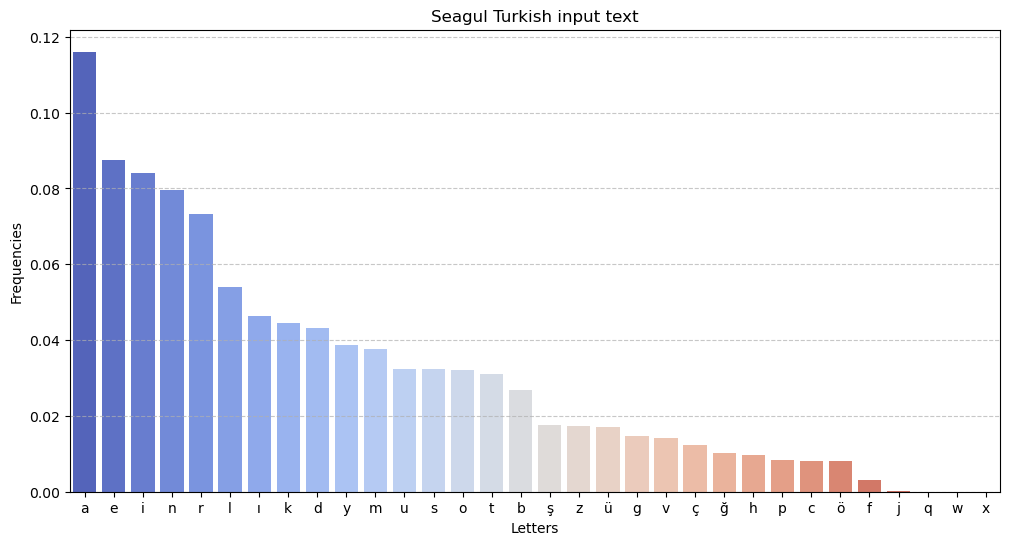
\includegraphics[width=\textwidth]{media/seagulTurkish.png} 
        \caption{Letter Frequency of Seagul in Turkish}
    \end{minipage}
    \hfill
    \begin{minipage}[b]{0.45\textwidth}
        \centering
        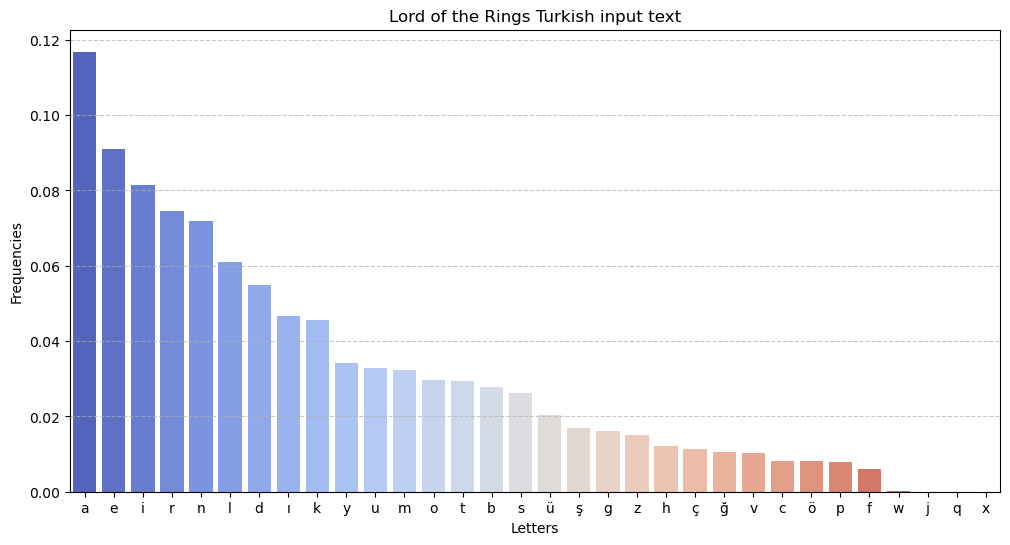
\includegraphics[width=\textwidth]{media/lordOfTheRingsTurkish.png}
        \caption{Letter Frequency of Lord of the Rings in Turkish}
    \end{minipage}
\end{figure}

\begin{figure}[htbp]
    \centering
    \begin{minipage}[b]{0.45\textwidth}
        \centering
        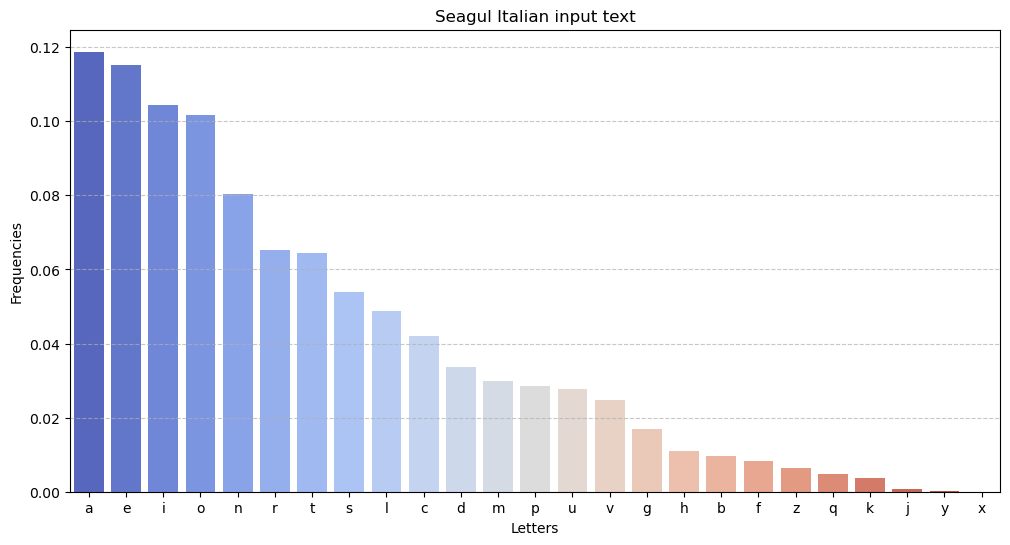
\includegraphics[width=\textwidth]{media/seagulItalian.png} 
        \caption{Letter Frequency of Seagul in Italian}
    \end{minipage}
    \hfill
    \begin{minipage}[b]{0.45\textwidth}
        \centering
        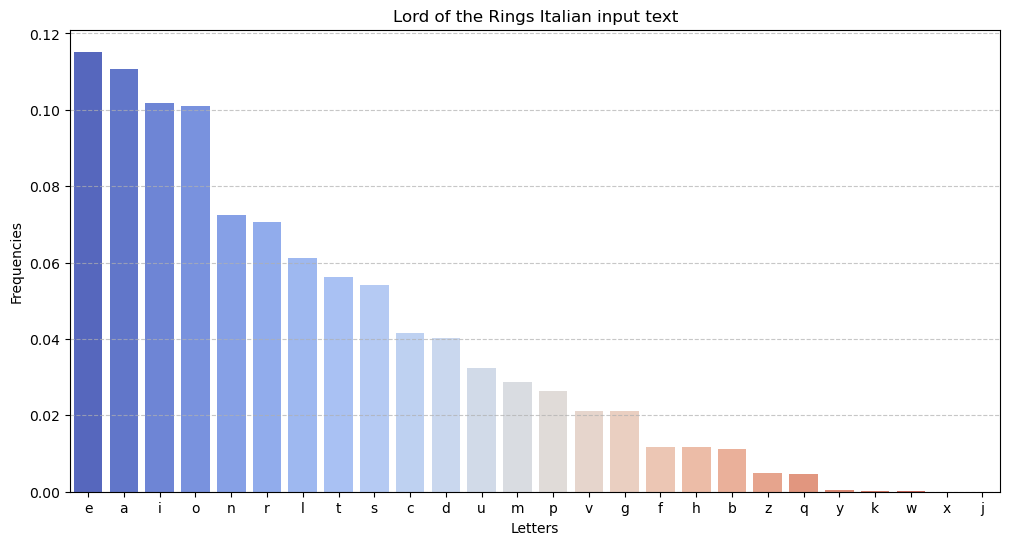
\includegraphics[width=\textwidth]{media/lordOfTheRingsItalian.png}
        \caption{Letter Frequency of Lord of the Rings in Italian}
    \end{minipage}
\end{figure}





\newpage
\subsection*{Comparison of small and medium datasets in each languages} 

\begin{figure}[h]
    \centering
    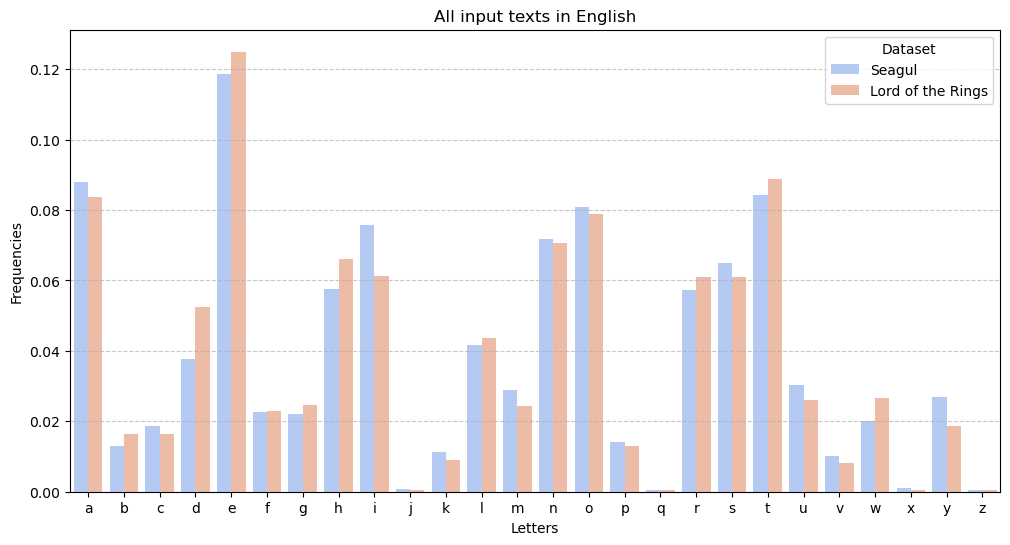
\includegraphics[width=0.6\textwidth]{media/allEnglish.png}
\end{figure}

\begin{figure}[h]
    \centering
    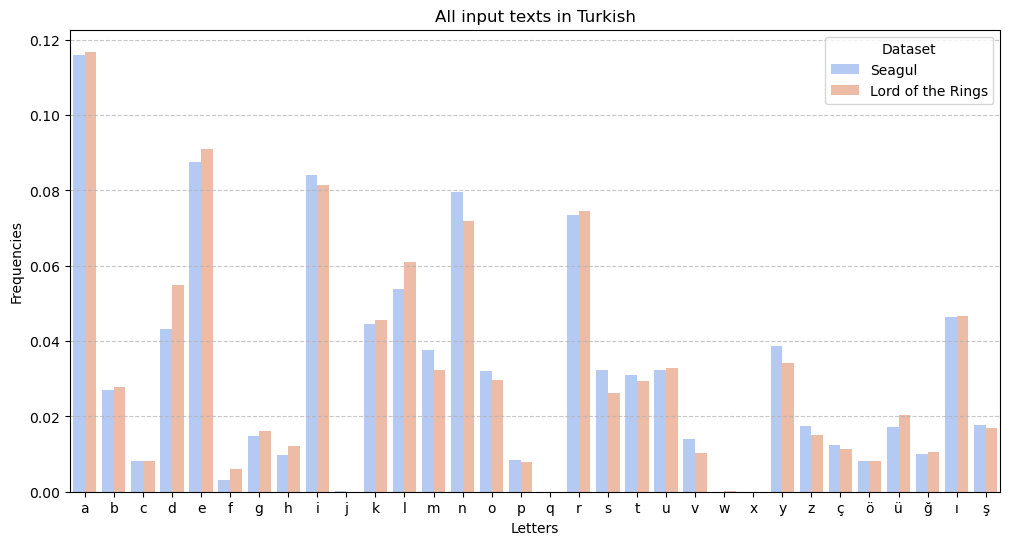
\includegraphics[width=0.6\textwidth]{media/allTurkish.png}
\end{figure}

\begin{figure}[h]
    \centering
    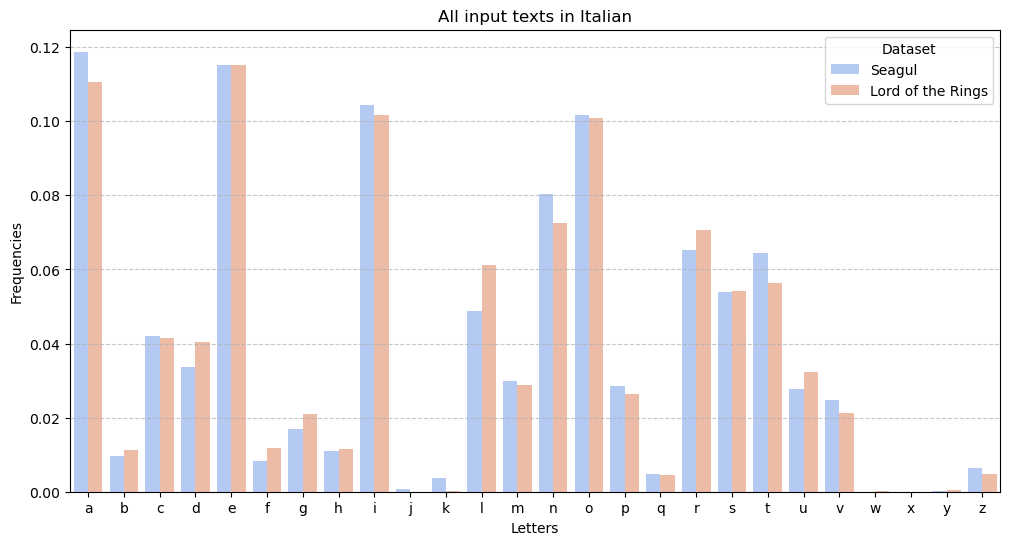
\includegraphics[width=0.6\textwidth]{media/allItalian.png}
\end{figure}


\textbf{Obtanied Results:}
\begin{itemize}
    \item In each language \textit{A} and \text{E} are the most frequent letters.
    \item \textit{T} has significantly more priority in English than the other languages.
    \item The frequency order of the letter in the same language is almost the same for the small and medium dataset.
    \item \textit{Q} and \textit{X} are the common few frequent letters in all languages.
    \item In general the vowel of the languages are more frequent than the consonants.
\end{itemize}